\documentclass{article}

\usepackage[T1]{fontenc}
\usepackage{libertine}

\usepackage{fancyhdr}
\usepackage{extramarks}
\usepackage{amsmath}
\usepackage{amsthm}
\usepackage{amsfonts}
\usepackage{tikz}
\usepackage{algorithm}
\usepackage{algpseudocode}
\usepackage{enumitem}

\usetikzlibrary{automata,positioning}

%
% Basic Document Settings
%

\topmargin=-0.45in
\evensidemargin=0in
\oddsidemargin=0in
\textwidth=6.5in
\textheight=9.0in
\headsep=0.25in

\linespread{1.1}

\pagestyle{fancy}
\lhead{\hmwkAuthorName}
\chead{\hmwkClass: \hmwkTitle}
\rhead{\firstxmark}
\lfoot{\lastxmark}
\cfoot{\thepage}

\renewcommand\headrulewidth{0.4pt}
\renewcommand\footrulewidth{0.4pt}

\setlength\parindent{0pt}

%
% Create Problem Sections
%

\newcommand{\enterProblemHeader}[1]{
    \nobreak\extramarks{}{Problem \arabic{#1} continued on next page\ldots}\nobreak{}
    \nobreak\extramarks{Problem \arabic{#1} (continued)}{Problem \arabic{#1} continued on next page\ldots}\nobreak{}
}

\newcommand{\exitProblemHeader}[1]{
    \nobreak\extramarks{Problem \arabic{#1} (continued)}{Problem \arabic{#1} continued on next page\ldots}\nobreak{}
    \stepcounter{#1}
    \nobreak\extramarks{Problem \arabic{#1}}{}\nobreak{}
}

\setcounter{secnumdepth}{0}
\newcounter{partCounter}
\newcounter{homeworkProblemCounter}
\setcounter{homeworkProblemCounter}{1}
\nobreak\extramarks{Problem \arabic{homeworkProblemCounter}}{}\nobreak{}

%
% Homework Problem Environment
%
% This environment takes an optional argument. When given, it will adjust the
% problem counter. This is useful for when the problems given for your
% assignment aren't sequential. See the last 3 problems of this template for an
% example.
%
\newenvironment{homeworkProblem}[1][-1]{
    \ifnum#1>0
        \setcounter{homeworkProblemCounter}{#1}
    \fi
    \section{Problem \arabic{homeworkProblemCounter}}
    \setcounter{partCounter}{1}
    \enterProblemHeader{homeworkProblemCounter}
}{
    \exitProblemHeader{homeworkProblemCounter}
}

%
% Homework Details
%   - Title
%   - Due date
%   - Class
%   - Section/Time
%   - Instructor
%   - Author
%

\newcommand{\hmwkTitle}{Homework\ \#2}
\newcommand{\hmwkDueDate}{February 15, 2018}
\newcommand{\hmwkClass}{Design and Analysis of Algorithms}
\newcommand{\hmwkClassInstructor}{Professor Kasturi Varadarajan}
\newcommand{\hmwkAuthorName}{\textbf{Alic Szecsei}}

%
% Title Page
%

\title{
    \vspace{2in}
    \textmd{\textbf{\hmwkClass:\ \hmwkTitle}}\\
    \normalsize\vspace{0.1in}\small{Due\ in\ class\ on\ \hmwkDueDate}\\
    \vspace{0.1in}\large{\textit{\hmwkClassInstructor}}
    \vspace{3in}
}

\author{\hmwkAuthorName}
\date{}

\renewcommand{\part}[1]{\textbf{\large Part \Alph{partCounter}}\stepcounter{partCounter}\\}

%
% Various Helper Commands
%

% Useful for algorithms
\newcommand{\alg}[1]{\textsc{\bfseries \footnotesize #1}}

% For derivatives
\newcommand{\deriv}[1]{\frac{\mathrm{d}}{\mathrm{d}x} (#1)}

% For partial derivatives
\newcommand{\pderiv}[2]{\frac{\partial}{\partial #1} (#2)}

% Integral dx
\newcommand{\dx}{\mathrm{d}x}

% Alias for the Solution section header
\newcommand{\solution}{\textbf{\large Solution}}

% Probability commands: Expectation, Variance, Covariance, Bias
\newcommand{\E}{\mathrm{E}}
\newcommand{\Var}{\mathrm{Var}}
\newcommand{\Cov}{\mathrm{Cov}}
\newcommand{\Bias}{\mathrm{Bias}}

% Set from 1 to N
\newcommand{\XYZ}[1]{\left\{1,\ldots,{#1}\right\}}

\begin{document}

\maketitle

\pagebreak

\begin{homeworkProblem}
Suppose we are given an array $A[1..n]$ with the special property that $A[1] \geq A[2]$ and $A[n-1] \leq A[n]$. We say that an element $A[x]$ is a \emph{local minimum} if it is less than or equal to both its neighbors, or more formally, if $A[x-1] \geq A[x]$ and $A[x] \leq A[x+1]$. For example, there are six local minima in the following array:\\
\begin{table}[h]
	\centering
	\begin{tabular}{ | *{15}{c |} c | }
		\hline
		9 & \textbf{7} & 7 & 2 & \textbf{1} & 3 & 7 & 5 & \textbf{4} & 7 & \textbf{3} & \textbf{3} & 4 & 8 & \textbf{6} & 9 \\
		\hline
\end{tabular}
	\caption{Example array}
	\label{tab:ExampleArray}
\end{table}

We can obviously find a local minimum in $O(n)$ time by scanning through the array. Describe and analyze an algorithm that finds a local minimum in $O(\log n)$ time. \emph{[Hint: With the given boundary conditions, the array \textbf{must} have at least one local minimum. Why?]}\\

\solution

\begin{algorithm}
	\caption{Algorithm for finding a local minimum}
	\label{algo:LocalMinimum}
	\begin{algorithmic}[1]
		\Function{FindLocalMinimum}{$A[1..n]$}
			\State{$median \gets n/2$}
			\If{$A[median] > A[median-1]$}
				\State{\Return{\Call{FindLocalMinimum}{$A[1..n/2]$}}}
			\ElsIf{$A[median] > A[median+1]$}
				\State{\Return{\Call{FindLocalMinimum}{$A[n/2..n]$}}}
			\Else{}
				\State{\Return{$median$}}
			\EndIf{}
		\EndFunction{}
	\end{algorithmic}
\end{algorithm}

Given the boundary conditions, the array \textbf{must} have at least one local minimum. To prove this, we can assume that the array has no local minimum. This means that the array must be either always increase or always decrease throughout the array; formally, $\forall x \in \XYZ{n}$, $A[x] > A[x-1]$ or $\forall x \in \XYZ{n}$, $A[x] > A[x+1]$. However since $A[1] \geq A[2]$ and $A[n-1] \leq A[n]$, this cannot be true; specifically it must \emph{start} by decreasing such that $A[x-1] \geq A[x]$ and then, at some point, stop decreasing, such that $A[x] \leq A[x+1]$. This point is the local minimum, since $A[x-1] \geq A[x] \leq A[x+1]$.\\

Given some median point, $m$, we can detect whether our array is increasing or decreasing at that point by examining the neighboring points. If the array is increasing, $A[m] \geq A[m-1]$. We know that the array starts by decreasing, so it must have started increasing since then; thus we can narrow our search for the local minimum to the first half of the array.\\

If the array is decreasing, $A[m] \geq A[m+1]$. Since the array ends with an increase, we know it must start increasing at some point after the median; thus we can narrow our search to the last half of the array.\\

If neither of these options is true, we must be at either a local maximum or minimum. If we are at a local maximum, then $A[m] \geq A[m-1]$, so we simply search the first half of the array; if we are at a local minimum, $A[m] \not> A[m+1]$ and $A[m] \not> A[m-1]$, so we reach our final branch and simply return $m$.

\end{homeworkProblem}

\begin{homeworkProblem}
Suppose we are given two sorted arrays $A[1..n]$ and $B[1..n]$ and an integer $k$. Describe an algorithm to find the $k$th smallest element in the union of $A$ and $B$ in $\Theta(\log n)$ time. For example, if $k = 1$, your algorithm should return the smallest element of $A \cup B$; if $k = n$, your algorithm should return the median of $A \cup B$. You can assume that the arrays contain no duplicate elements. \emph{[Hint: First solve the special case $k = n$.]}\\

\solution

\begin{algorithm}
	\caption{Algorithm for finding the $k$th smallest element in a union}
	\label{algo:kthSmallest}
	\begin{algorithmic}[1]
		\Function{FindKSmallest}{$A[1..m], B[1..n], k$}
			\If{$k = 1$}
				\If{$m = 0$}
					\State{\Return{$B[1]$}}
				\ElsIf{$n = 0$}
					\State{\Return{$A[1]$}}
				\Else{}
					\State{\Return{$min(A[1], B[1])$}}
				\EndIf{}
			\Else{}
				\State{$mid \gets \left\lfloor \frac{k}{2} \right\rfloor$}
				\If{$mid \geq m + 1$}
					\State{\Call{FindKSmallest}{$A, B[mid+1..n], k - mid$}}
				\ElsIf{$mid \geq n + 1$}
					\State{\Call{FindKSmallest}{$A[mid+1..m], B, k - mid$}}
				\ElsIf{$A[mid] < B[mid]$}
					\State{\Call{FindKSmallest}{$A[mid+1..m], B, k - mid$}}
				\Else{}
					\State{\Call{FindKSmallest}{$A, B[mid+1..n], k - mid$}}
				\EndIf{}
			\EndIf{}
		\EndFunction{}
	\end{algorithmic}
\end{algorithm}

As an example, we will run through the algorithm with $A = \{1, 3, 5, 7\}$ and $B = \{2, 4, 6, 8\}$, with $k = 4$.\\

Since $k \neq 1$, we determine a middle element, $mid = \left\lfloor \frac{k}{2} \right\rfloor = 2$. Since $mid < m + 1$ and $mid < n + 1$, we compare the second element of each array. $A$ has a smaller element, since $A[2] = 3 < B[2] = 4$, so we recurse with a new $A = \{5, 7\}$, $B$ remaining the same, and $k = k - mid = 4 - 2 = 2$.\\

$k$ is still not $1$, so we determine our middle element, $mid = \left\lfloor \frac{k}{2} \right\rfloor = 1$. Since $mid < m + 1$ and $mid < n + 1$, we compare the first element of each array. $B$ has a smaller element, since $B[1] = 2$, so we recurse with a new $B = \{4, 6, 8\}$, $A$ remaining the same, and $k = k - mid = 2 - 1 = 1$.\\

Now, $k = 1$. Since neither $A$ nor $B$ are empty, we simply find the minimum of their first elements; $B[1] = 4$ and $A[1] = 5$, so we return $4$, as expected.\\

In general, we can safely divide the two arrays into four sections: $A_1$, $A_2$, $B_1$, and $B_2$, such that $A_1$ and $B_1$ have length $\frac{k}{2}$. Since the arrays are sorted, we know that $A_1 < A_2$, and $B_1 < B_2$. Since we are looking for the $k$th smallest element, and $\left| A_1 \cup B_1 \right| = k$, it must either be the largest element of $A_1 \cup B_1$ or somewhere in $A_2 \cup B_2$.\\

We compare the last elements of $A_1$ and $B_1$ to determine which \emph{might} contain the $k$th smallest element, and can then safely discard the other. Since we have discarded elements smaller than the $k$th smallest, we update our value of $k$, removing the number of elements we discarded - $\frac{k}{2}$. We continue in this manner, discarding elements when possible, until we have reached our trivial base case, where $k = 1$ and we can simply find the minimal element of $A \cup B$.

\end{homeworkProblem}

\begin{homeworkProblem}
For this problem, a \emph{subtree} of a binary tree means any connected subgraph. A binary tree is \emph{complete} if every internal node has two children, and every leaf has exactly the same depth. Describe and analyze a recursive algorithm to compute the \emph{largest complete subtree} of a given binary tree. Your algorithm should return the root and the depth of this subtree.

\begin{figure}[h]
	\centering
		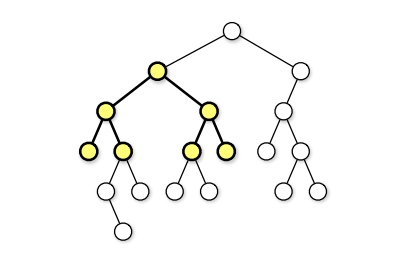
\includegraphics{images/binary-subtree.png}
	\caption{The largest complete subtree of this binary tree has depth 2.}
	\label{fig:binary-subtree}
\end{figure}

\solution

\begin{algorithm}
	\caption{Algorithm for finding the largest complete subtree}
	\label{algo:largestcomplete}
	\begin{algorithmic}[1]
		\Function{LargestCompleteSubtree}{$root$}
			
		\EndFunction{}
	\end{algorithmic}
\end{algorithm}

\end{homeworkProblem}

\begin{homeworkProblem}
\begin{enumerate}[label=(\alph*)]
	\item Let $A[1..m]$ and $B[1..n]$ be two arbitrary arrays. A \emph{common subsequence} of $A$ and $B$ is both a subsequence of $A$ and a subsequence of $B$. Give a simple recursive definition for the function $lcs(A,B)$, which gives the length of the \emph{longest} common subsequence of $A$ and $B$.
	\item Call a sequence $X[1..n]$ \emph{oscillating} if $X[i] < X[i+1]$ for all even $i$, and $X[i] > X[i+1]$ for all odd $i$. Give a simple recursive definition for the function $los(A)$, which gives the length of the longest oscillating subsequence of an arbitrary array $A$ of integers.
	\item Call a sequence $X[1..n]$ \emph{accelerating} if $2 \times X[i] < X[i-1] + X[i+1]$ for all $i$. Give a simple recursive definition for the function $lxs(A)$, which gives the length of the longest accelerating subsequence of an arbitrary array $A$ of integers.
\end{enumerate}

\solution



\end{homeworkProblem}

\end{document}